\subsection{Event-baseret beskedsystem}
Til at kommunikere mellem tråde benyttes et event-baseres beskedsystem. Det fungerer ved, at tråde hele tiden lytter efter beskeder, og når der kommer en besked, håndteres den, før tråden igen lytter efter næste besked.

\begin{figure}[H]
    \centering
    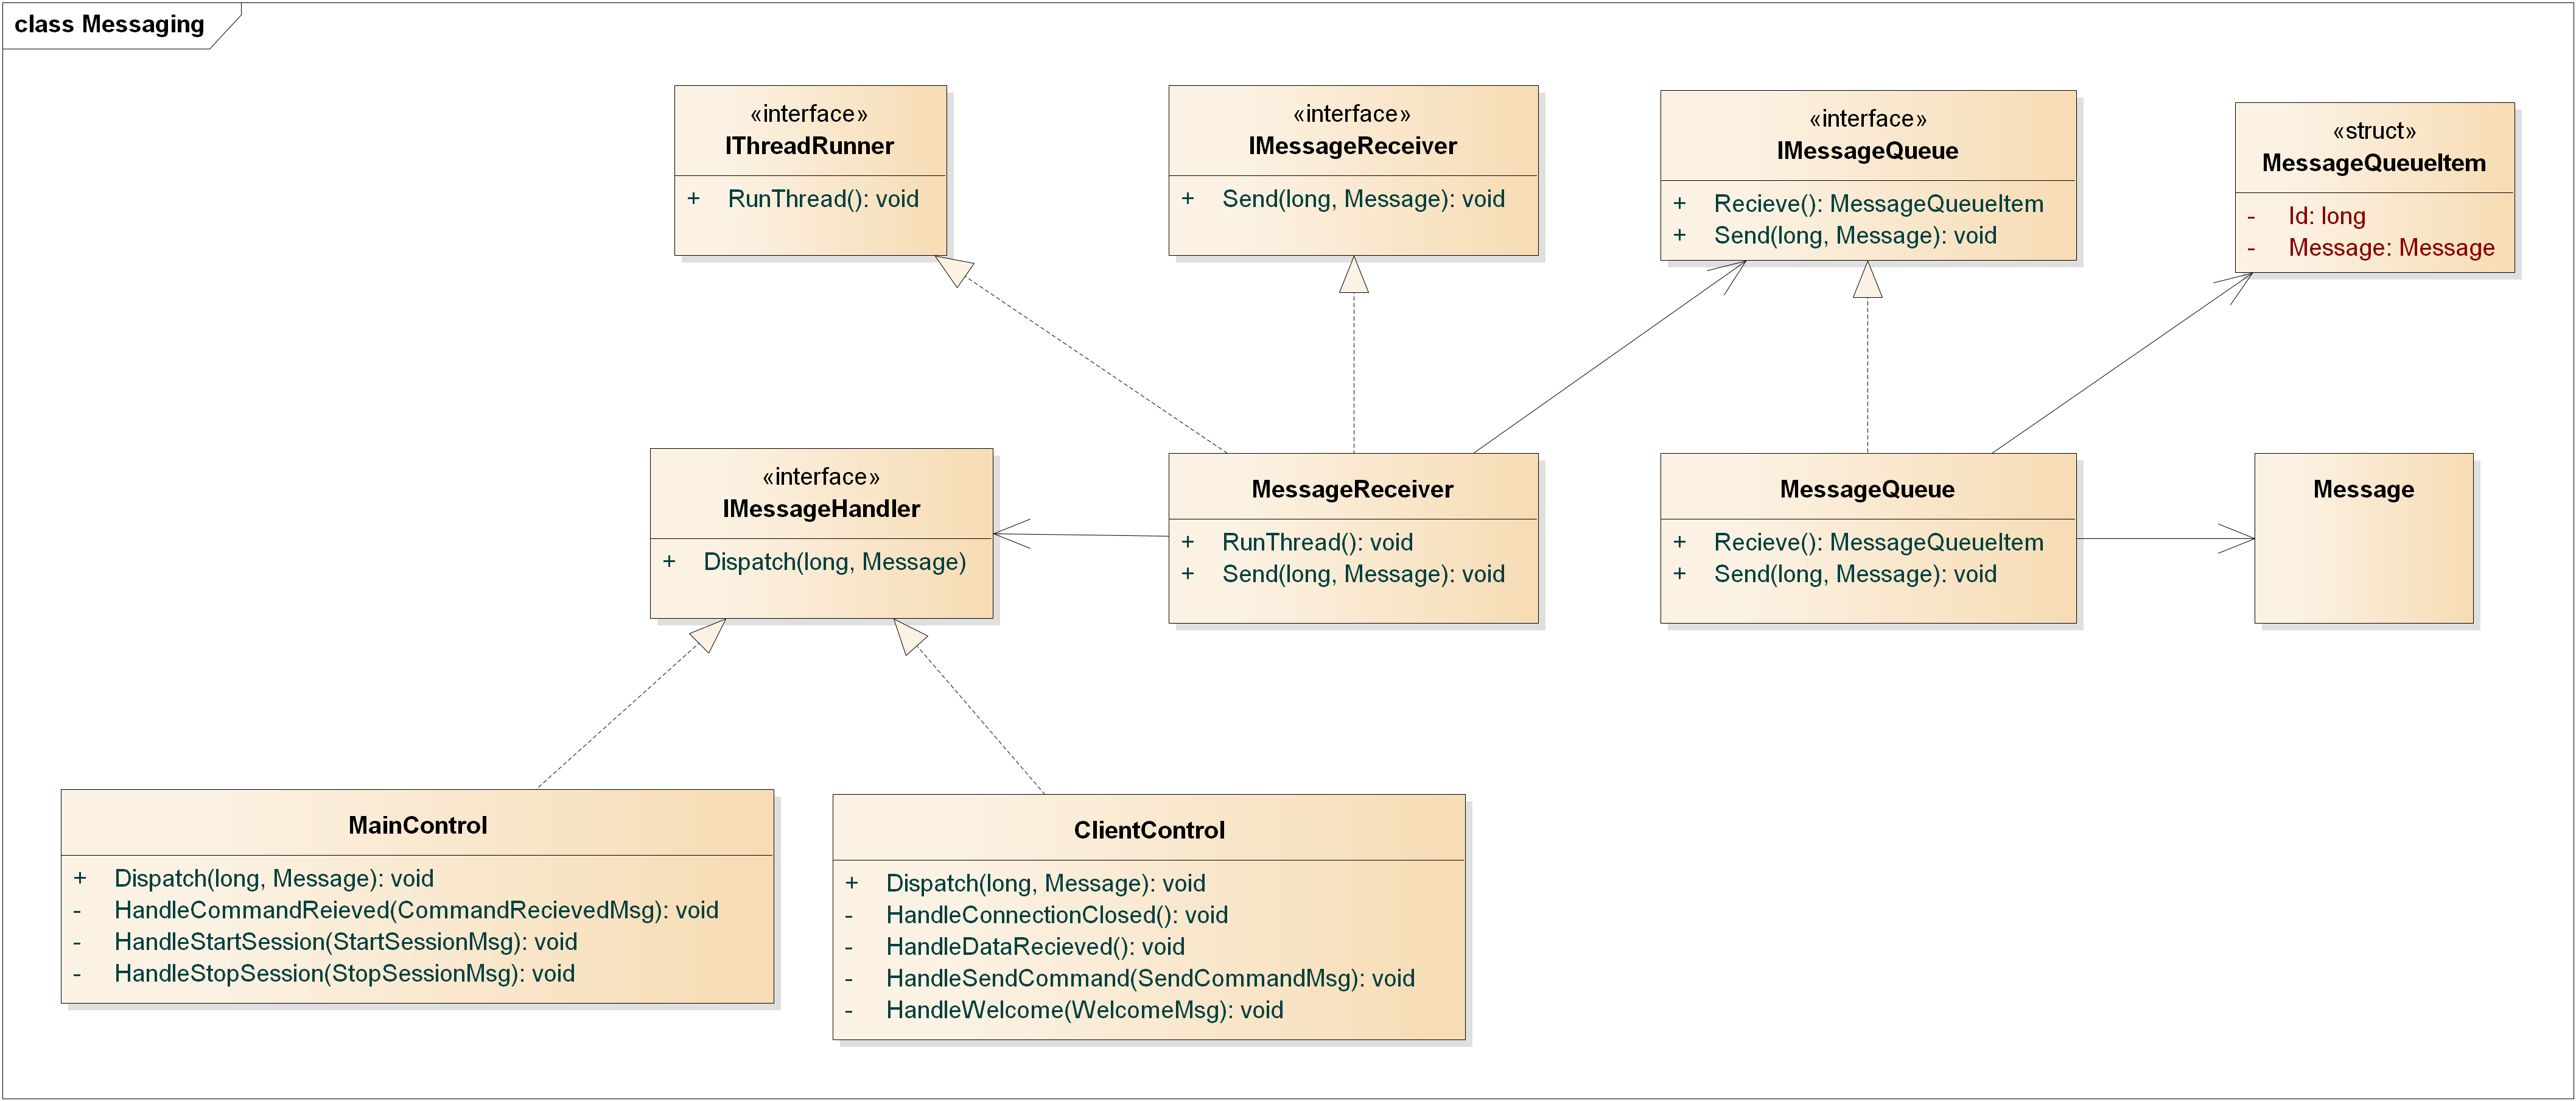
\includegraphics[width=1\textwidth]{Systemdesign/CentralServer/Images/Beskedsystem.png}
    \caption{UML-diagram for Messaging pakken}
    \label{fig:CSBeskedsystem}
\end{figure}


\textbf{Modtagere}\\
For at implementere en beskedmodtager, laver man en instans af klassen MessageReceiver. Klassen benytter sig af et objekt, som implementerer interfacet MessageHandler, til at håndtere beskeder. I CentralServer er det pt. kun MainControl og ClientControl, som benytter denne funktionalitet, da det kun er disse to tråde, som skal kunne modtage beskeder.\\

\textbf{Beskedkø}\\
MessageReceiver læser beskeder fra en beskedkø, som er implementeret i interfacet IMessageQueue. Køen fungerer som en FIFO-kø. Trådsynkronisering foregår i denne klasse.\\

\textbf{Beskeder}\\
En besked mellem to tråde består af to ting: et event id og et Message objekt (sidstnævnte er valgfri). Tilgængelige event id’er bestemmes altid af modtageren. Message objektet indeholder de data, som skal sendes mellem trådene, og der findes unikke objekter for hver besked, alt efter hvilket data, der kræves til den enkelte kommando.\\

Figur \ref{fig:CSBeskeder} viser hirakiet af beskeder.

\begin{figure}[H]
    \centering
    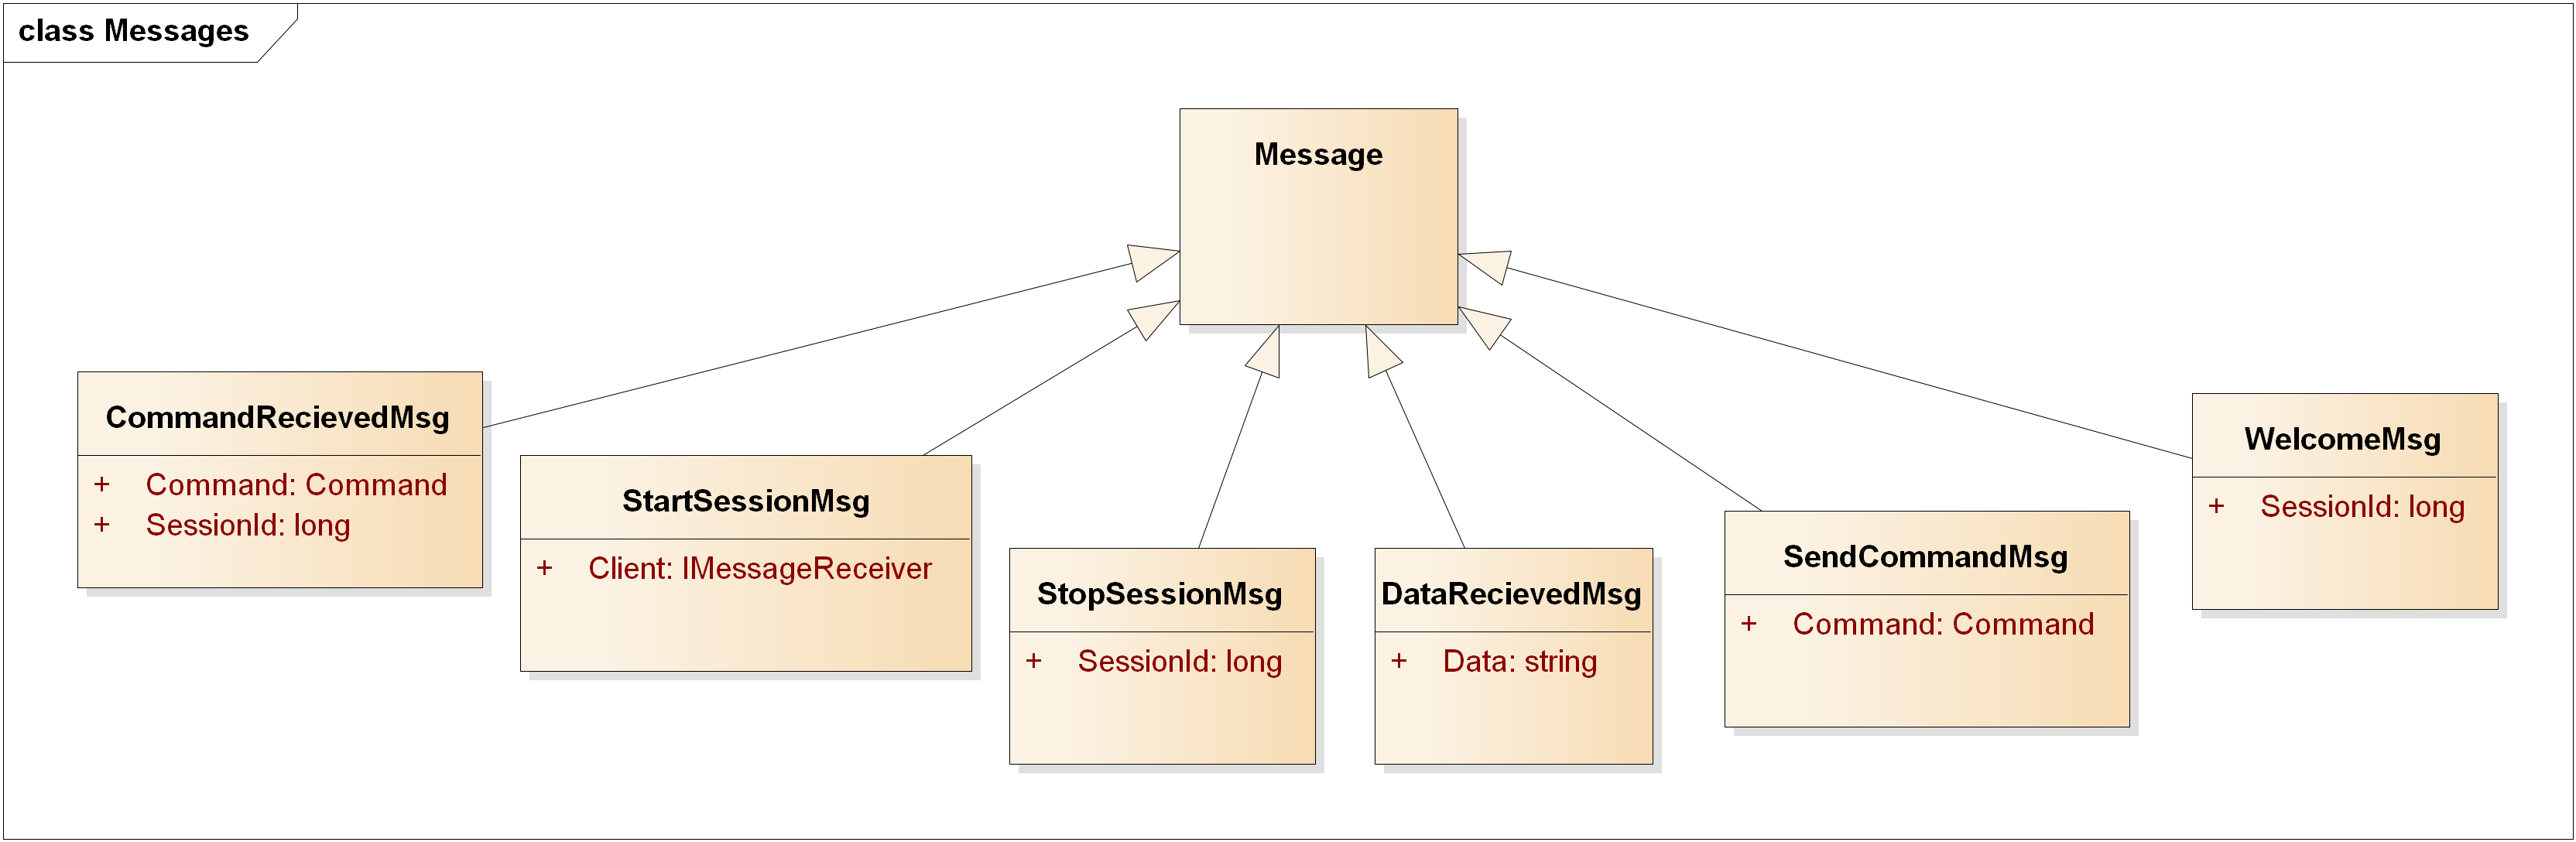
\includegraphics[width=1\textwidth]{Systemdesign/CentralServer/Images/Beskeder.png}
    \caption{UML-diagram for beskeder}
    \label{fig:CSBeskeder}
\end{figure}


\textbf{Modtagelse af beskeder}\\
Nedenfor ses, hvordan modtagelse af beskeder foregår. I diagrammet kan ”Message sender” være enten MainControl eller ClientControl, og IMessageHandler kan være enten MainControl eller ClientControl.\\

Figur \ref{fig:CSModtagelseAfBeskeder} viser sekvensen for modtagelse og behandling af beskeder.

\begin{figure}[H]
    \centering
    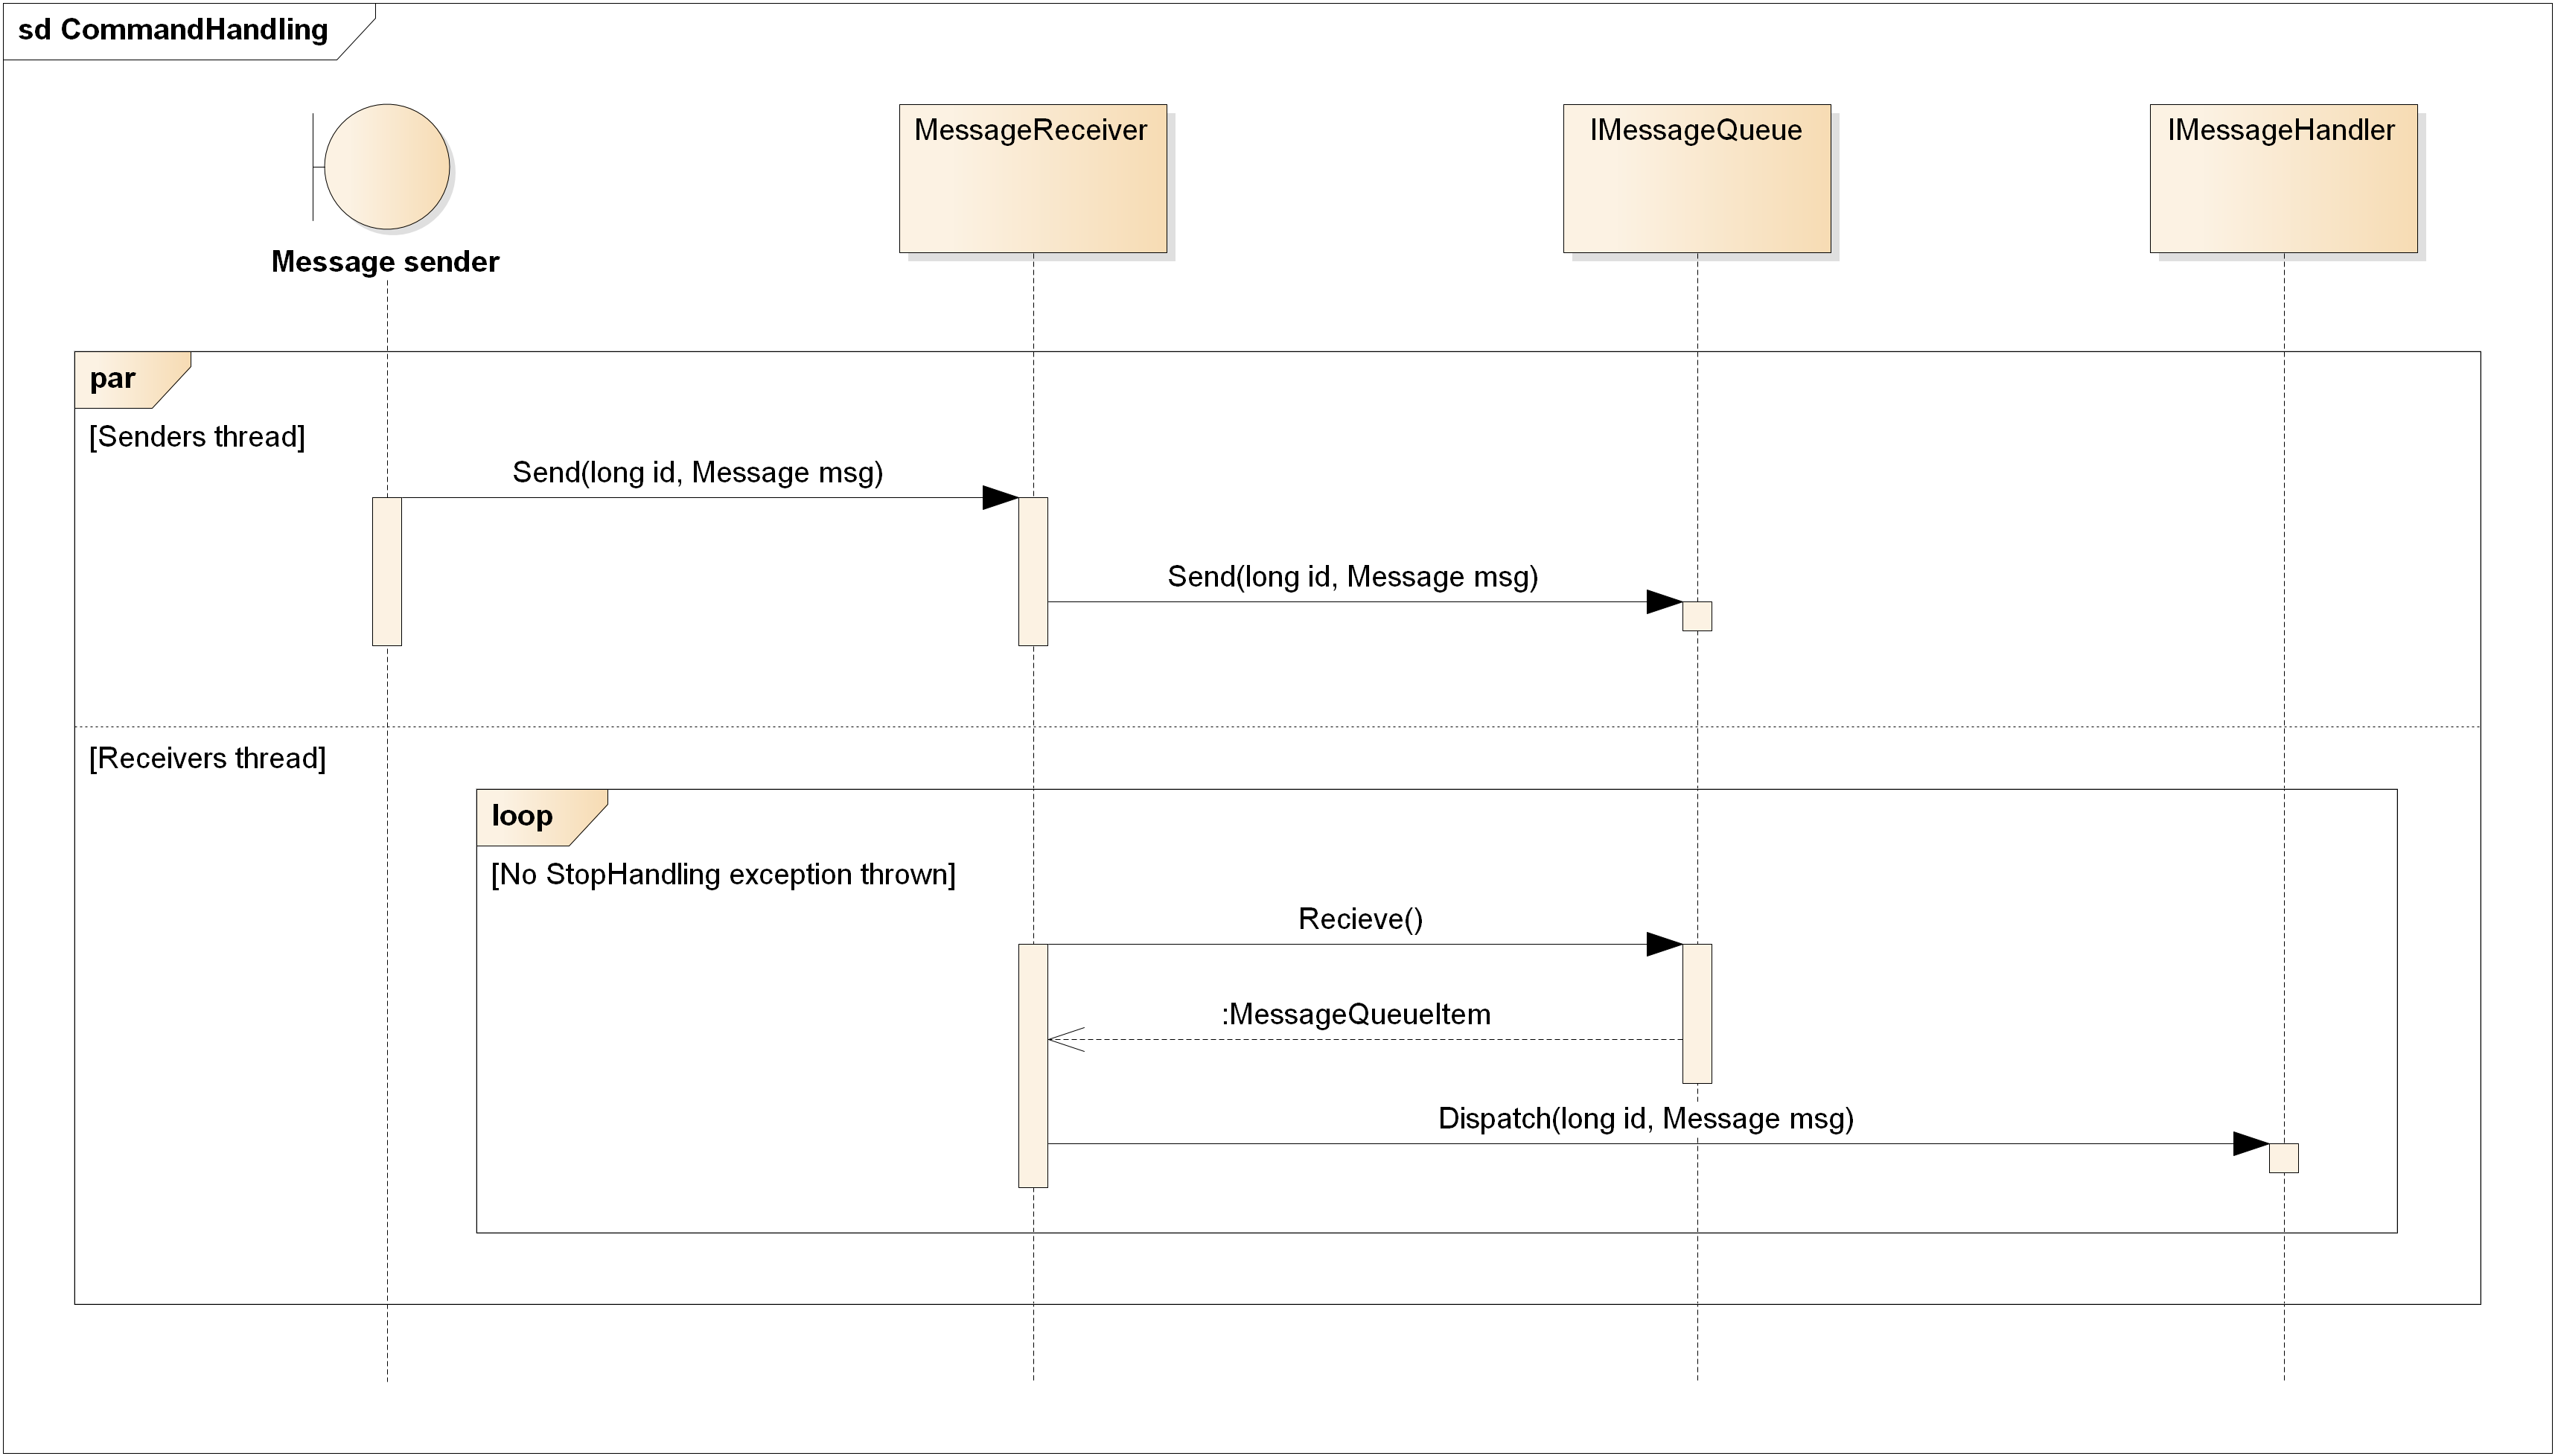
\includegraphics[width=1\textwidth]{Systemdesign/CentralServer/Images/ModtagelseAfBeskeder.png}
    \caption{Sekvensdiagrammet viser, hvordan modtagelse af beskeder håndteres}
    \label{fig:CSModtagelseAfBeskeder}
\end{figure}